\centerline{19.03.2025}


\centerline{\bf \large Региональный этап XVII  республиканской математической олимпиады}
\centerline{\bf \large  школьников  имени академика РАО  П.М. Эрдниева  }

\centerline{\bf \Large  4 класс}

\problem{\textbf{1}} Пюрвя Мучкаевич придумал систему перевода цифр в буквы и обратно, в которой каждой из десяти цифр соответствует одна уникальная буква. Он решил воспользоваться новой системой и сложил в столбик два слова УДЕ + УДЕ. Мог ли Пюрвя Мучкаевич получить в результате слово НАУКА? Если мог, то приведите пример таких чисел, если нет, то объясните почему.

\problem{\textbf{2}} Решите задачу:

а) Батыр и Очир вместе решают сборник 720 удивительных заданий Пюрви Мучкаевича за 40 дней. За сколько дней решит этот сборник один Батыр, если он за 4 дня решает столько же заданий, сколько Очир за 5 дней?

Батыр решает сборник 720 удивительных заданий Пюрви Мучкаевича за 72 дня. За сколько дней решат этот сборник Батыр вместе с Очиром, если Батыр за 4 дня решает столько же заданий, сколько Очир за 5 дней?

б) Составьте и решите обратную задачу по схеме: 720; ?; 72; 4; 5.


\problem{\textbf{3}} В степи паслись 25 коров. Пастухи пригнали стадо овец. Овец оказалось больше, чем у коров ушей, но меньше, чем у коров ног. Сколько было овец, если их в 25 раз больше, чем пастухов?

\problem{\textbf{4}} Разрежьте фигуру, изображённую на рисунке снизу, по клеточкам на три
нераспадающиеся части так, чтобы из них можно было сложить квадрат (поворачивать части можно, переворачивать нельзя).

\begin{center}
    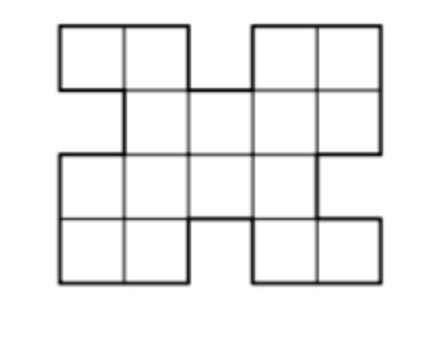
\includegraphics[width=0.2\textwidth]{Секретная информация/УДЕ 2024-2025/Регион. Условия/4.4.png}
\end{center}

\problem{\textbf{5}} Фигура \textit{Сайгак} бьёт все клетки, находящиеся от неё через клетку слева, справа, сверху или снизу, а также бьёт клетку, на которой стоит. Какое наименьшее количество \textit{Сайгаков} необходимо поставить на клетчатую доску 8 × 8 , чтобы эти фигуры били все клетки доски?


\centerline{\bf }


\centerline{\bf  Желаем удачи!}
\centerline{\bf  Время на выполнение 180 минут.}


\includegraphics[width=5cm]{Секретная информация/УДЕ 2024-2025/QR_code.jpg} % Левая картинка
    \hfill
    \textbf{Разбор в 15:00 по QR - коду слева.}
    \hfill

\includegraphics[width=5cm]{Секретная информация/УДЕ 2024-2025/logo_ude.png} % Правая картинка